\chapter{Sắp xếp}

\index{sắp xếp}

\key{Sắp xếp}
là một bài toán thiết kế thuật toán cơ bản.
Nhiều thuật toán hiệu quả
sử dụng sắp xếp như một chương trình con,
bởi vì việc xử lý dữ liệu thường dễ dàng hơn
nếu các phần tử đã ở theo thứ tự được sắp xếp.

Ví dụ, bài toán ''một mảng có chứa
hai phần tử bằng nhau không?'' rất dễ giải quyết bằng cách sử dụng sắp xếp.
Nếu mảng chứa hai phần tử bằng nhau,
chúng sẽ nằm cạnh nhau sau khi sắp xếp,
vì vậy rất dễ để tìm thấy chúng.
Ngoài ra, bài toán ''phần tử nào xuất hiện thường xuyên nhất
trong một mảng?'' cũng có thể được giải quyết tương tự.

Có rất nhiều thuật toán để sắp xếp, và chúng cũng
là những ví dụ điển hình về cách áp dụng
các kỹ thuật thiết kế thuật toán khác nhau.
Các thuật toán sắp xếp tổng quát hiệu quả
hoạt động trong thời gian $O(n \log n)$,
và nhiều thuật toán sử dụng sắp xếp
như một chương trình con cũng
có độ phức tạp thời gian này.

\section{Lý thuyết sắp xếp}

Bài toán cơ bản trong sắp xếp như sau:
\begin{framed}
\noindent
Cho một mảng chứa $n$ phần tử,
nhiệm vụ của bạn là sắp xếp các phần tử
theo thứ tự tăng dần.
\end{framed}
\noindent
Ví dụ, mảng
\begin{center}
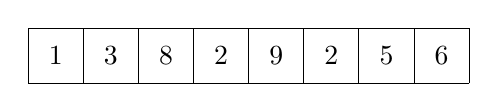
\begin{tikzpicture}[scale=0.7]
\draw (0,0) grid (8,1);
\node at (0.5,0.5) {$1$};
\node at (1.5,0.5) {$3$};
\node at (2.5,0.5) {$8$};
\node at (3.5,0.5) {$2$};
\node at (4.5,0.5) {$9$};
\node at (5.5,0.5) {$2$};
\node at (6.5,0.5) {$5$};
\node at (7.5,0.5) {$6$};
\end{tikzpicture}
\end{center}
sẽ trở thành như sau sau khi sắp xếp:
\begin{center}
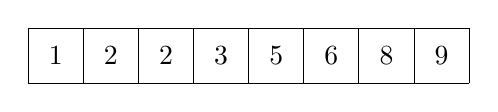
\begin{tikzpicture}[scale=0.7]
\draw (0,0) grid (8,1);
\node at (0.5,0.5) {$1$};
\node at (1.5,0.5) {$2$};
\node at (2.5,0.5) {$2$};
\node at (3.5,0.5) {$3$};
\node at (4.5,0.5) {$5$};
\node at (5.5,0.5) {$6$};
\node at (6.5,0.5) {$8$};
\node at (7.5,0.5) {$9$};
\end{tikzpicture}
\end{center}

\subsubsection{Các thuật toán $O(n^2)$}

\index{sắp xếp nổi bọt}

Các thuật toán đơn giản để sắp xếp một mảng
hoạt động trong thời gian $O(n^2)$.
Các thuật toán như vậy thường ngắn và
bao gồm hai vòng lặp lồng nhau.
Một thuật toán sắp xếp thời gian $O(n^2)$ nổi tiếng
là \key{sắp xếp nổi bọt} (bubble sort), trong đó các phần tử
''nổi bọt'' trong mảng theo giá trị của chúng.

Sắp xếp nổi bọt bao gồm $n$ vòng.
Ở mỗi vòng, thuật toán lặp qua
các phần tử của mảng.
Bất cứ khi nào tìm thấy hai phần tử liên tiếp
không đúng thứ tự,
thuật toán sẽ hoán đổi chúng.
Thuật toán có thể được cài đặt như sau:
\begin{lstlisting}
for (int i = 0; i < n; i++) {
    for (int j = 0; j < n-1; j++) {
        if (array[j] > array[j+1]) {
            swap(array[j],array[j+1]);
        }
    }
}
\end{lstlisting}

Sau vòng đầu tiên của thuật toán,
phần tử lớn nhất sẽ ở đúng vị trí,
và nói chung, sau $k$ vòng, $k$ phần tử
lớn nhất sẽ ở đúng vị trí của chúng.
Do đó, sau $n$ vòng, toàn bộ mảng
sẽ được sắp xếp.

Ví dụ, trong mảng

\begin{center}
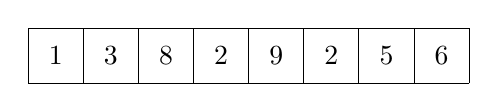
\begin{tikzpicture}[scale=0.7]
\draw (0,0) grid (8,1);

\node at (0.5,0.5) {$1$};
\node at (1.5,0.5) {$3$};
\node at (2.5,0.5) {$8$};
\node at (3.5,0.5) {$2$};
\node at (4.5,0.5) {$9$};
\node at (5.5,0.5) {$2$};
\node at (6.5,0.5) {$5$};
\node at (7.5,0.5) {$6$};
\end{tikzpicture}
\end{center}

\noindent
vòng đầu tiên của sắp xếp nổi bọt sẽ hoán đổi các phần tử
như sau:

\begin{center}
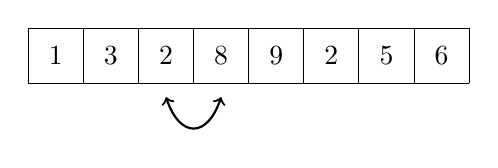
\begin{tikzpicture}[scale=0.7]
\draw (0,0) grid (8,1);
\node at (0.5,0.5) {$1$};
\node at (1.5,0.5) {$3$};
\node at (2.5,0.5) {$2$};
\node at (3.5,0.5) {$8$};
\node at (4.5,0.5) {$9$};
\node at (5.5,0.5) {$2$};
\node at (6.5,0.5) {$5$};
\node at (7.5,0.5) {$6$};

\draw[thick,<->] (3.5,-0.25) .. controls (3.25,-1.00) and (2.75,-1.00) .. (2.5,-0.25);
\end{tikzpicture}
\end{center}

\begin{center}
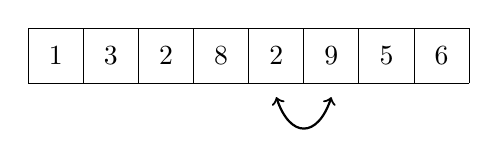
\begin{tikzpicture}[scale=0.7]
\draw (0,0) grid (8,1);
\node at (0.5,0.5) {$1$};
\node at (1.5,0.5) {$3$};
\node at (2.5,0.5) {$2$};
\node at (3.5,0.5) {$8$};
\node at (4.5,0.5) {$2$};
\node at (5.5,0.5) {$9$};
\node at (6.5,0.5) {$5$};
\node at (7.5,0.5) {$6$};

\draw[thick,<->] (5.5,-0.25) .. controls (5.25,-1.00) and (4.75,-1.00) .. (4.5,-0.25);
\end{tikzpicture}
\end{center}

\begin{center}
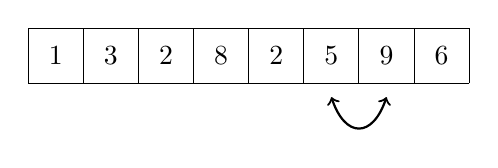
\begin{tikzpicture}[scale=0.7]
\draw (0,0) grid (8,1);
\node at (0.5,0.5) {$1$};
\node at (1.5,0.5) {$3$};
\node at (2.5,0.5) {$2$};
\node at (3.5,0.5) {$8$};
\node at (4.5,0.5) {$2$};
\node at (5.5,0.5) {$5$};
\node at (6.5,0.5) {$9$};
\node at (7.5,0.5) {$6$};

\draw[thick,<->] (6.5,-0.25) .. controls (6.25,-1.00) and (5.75,-1.00) .. (5.5,-0.25);
\end{tikzpicture}
\end{center}

\begin{center}
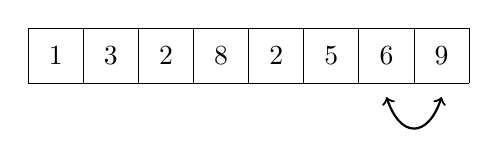
\begin{tikzpicture}[scale=0.7]
\draw (0,0) grid (8,1);
\node at (0.5,0.5) {$1$};
\node at (1.5,0.5) {$3$};
\node at (2.5,0.5) {$2$};
\node at (3.5,0.5) {$8$};
\node at (4.5,0.5) {$2$};
\node at (5.5,0.5) {$5$};
\node at (6.5,0.5) {$6$};
\node at (7.5,0.5) {$9$};

\draw[thick,<->] (7.5,-0.25) .. controls (7.25,-1.00) and (6.75,-1.00) .. (6.5,-0.25);
\end{tikzpicture}
\end{center}

\subsubsection{Nghịch thế}

\index{nghịch thế}

Sắp xếp nổi bọt là một ví dụ về thuật toán
sắp xếp luôn hoán đổi các phần tử \emph{liên tiếp}
trong mảng.
Hóa ra độ phức tạp thời gian
của một thuật toán như vậy là \emph{luôn luôn}
ít nhất là $O(n^2)$, bởi vì trong trường hợp xấu nhất,
cần $O(n^2)$ lần hoán đổi để sắp xếp mảng.

Một khái niệm hữu ích khi phân tích các thuật toán
sắp xếp là \key{nghịch thế}:
một cặp phần tử của mảng
$(\texttt{array}[a],\texttt{array}[b])$ sao cho
$a<b$ và $\texttt{array}[a]>\texttt{array}[b]$,
tức là, các phần tử đang ở sai thứ tự.
Ví dụ, mảng
\begin{center}
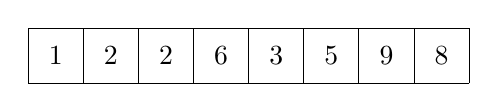
\begin{tikzpicture}[scale=0.7]
\draw (0,0) grid (8,1);
\node at (0.5,0.5) {$1$};
\node at (1.5,0.5) {$2$};
\node at (2.5,0.5) {$2$};
\node at (3.5,0.5) {$6$};
\node at (4.5,0.5) {$3$};
\node at (5.5,0.5) {$5$};
\node at (6.5,0.5) {$9$};
\node at (7.5,0.5) {$8$};
\end{tikzpicture}
\end{center}
có ba nghịch thế: $(6,3)$, $(6,5)$ và $(9,8)$.
Số lượng nghịch thế cho biết
cần bao nhiêu công sức để sắp xếp mảng.
Một mảng được sắp xếp hoàn toàn khi
không có nghịch thế nào.
Mặt khác, nếu các phần tử mảng
được sắp xếp theo thứ tự ngược lại,
số lượng nghịch thế là lớn nhất có thể:
\[1+2+\cdots+(n-1)=\frac{n(n-1)}{2} = O(n^2)\]

Hoán đổi một cặp phần tử liên tiếp đang
ở sai thứ tự sẽ loại bỏ chính xác một nghịch thế
khỏi mảng.
Do đó, nếu một thuật toán sắp xếp chỉ có thể
hoán đổi các phần tử liên tiếp, mỗi lần hoán đổi sẽ loại bỏ
nhiều nhất một nghịch thế, và độ phức tạp thời gian
của thuật toán ít nhất là $O(n^2)$.

\subsubsection{Các thuật toán $O(n \log n)$}

\index{sắp xếp trộn}

Có thể sắp xếp một mảng một cách hiệu quả
trong thời gian $O(n \log n)$ bằng cách sử dụng các thuật toán
không bị giới hạn trong việc hoán đổi các phần tử liên tiếp.
Một thuật toán như vậy là \key{sắp xếp trộn} (merge sort)\footnote{Theo \cite{knu983},
sắp xếp trộn được phát minh bởi J. von Neumann vào năm 1945.},
dựa trên đệ quy.

Sắp xếp trộn sắp xếp một mảng con \texttt{array}$[a \ldots b]$ như sau:

\begin{enumerate}
\item Nếu $a=b$, không làm gì cả, vì mảng con đã được sắp xếp.
\item Tính vị trí của phần tử ở giữa: $k=\lfloor (a+b)/2 \rfloor$.
\item Sắp xếp đệ quy mảng con \texttt{array}$[a \ldots k]$.
\item Sắp xếp đệ quy mảng con \texttt{array}$[k+1 \ldots b]$.
\item \emph{Trộn} các mảng con đã sắp xếp \texttt{array}$[a \ldots k]$ và
\texttt{array}$[k+1 \ldots b]$
thành một mảng con đã sắp xếp \texttt{array}$[a \ldots b]$.
\end{enumerate}

Sắp xếp trộn là một thuật toán hiệu quả vì nó
chia đôi kích thước của mảng con ở mỗi bước.
Quá trình đệ quy bao gồm $O(\log n)$ cấp,
và việc xử lý mỗi cấp mất thời gian $O(n)$.
Việc trộn các mảng con \texttt{array}$[a \ldots k]$ và \texttt{array}$[k+1 \ldots b]$
có thể thực hiện trong thời gian tuyến tính, vì chúng đã được sắp xếp.

Ví dụ, hãy xem xét việc sắp xếp mảng sau:
\begin{center}
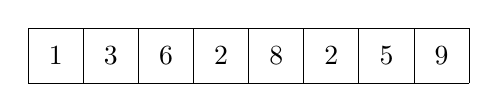
\begin{tikzpicture}[scale=0.7]
\draw (0,0) grid (8,1);
\node at (0.5,0.5) {$1$};
\node at (1.5,0.5) {$3$};
\node at (2.5,0.5) {$6$};
\node at (3.5,0.5) {$2$};
\node at (4.5,0.5) {$8$};
\node at (5.5,0.5) {$2$};
\node at (6.5,0.5) {$5$};
\node at (7.5,0.5) {$9$};
\end{tikzpicture}
\end{center}

Mảng sẽ được chia thành hai mảng con
như sau:
\begin{center}
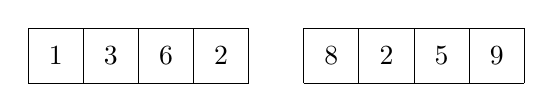
\begin{tikzpicture}[scale=0.7]
\draw (0,0) grid (4,1);
\draw (5,0) grid (9,1);

\node at (0.5,0.5) {$1$};
\node at (1.5,0.5) {$3$};
\node at (2.5,0.5) {$6$};
\node at (3.5,0.5) {$2$};

\node at (5.5,0.5) {$8$};
\node at (6.5,0.5) {$2$};
\node at (7.5,0.5) {$5$};
\node at (8.5,0.5) {$9$};
\end{tikzpicture}
\end{center}

Sau đó, các mảng con sẽ được sắp xếp đệ quy
như sau:
\begin{center}
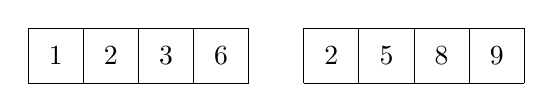
\begin{tikzpicture}[scale=0.7]
\draw (0,0) grid (4,1);
\draw (5,0) grid (9,1);

\node at (0.5,0.5) {$1$};
\node at (1.5,0.5) {$2$};
\node at (2.5,0.5) {$3$};
\node at (3.5,0.5) {$6$};

\node at (5.5,0.5) {$2$};
\node at (6.5,0.5) {$5$};
\node at (7.5,0.5) {$8$};
\node at (8.5,0.5) {$9$};
\end{tikzpicture}
\end{center}

Cuối cùng, thuật toán trộn các mảng con
đã sắp xếp và tạo ra mảng được sắp xếp cuối cùng:
\begin{center}
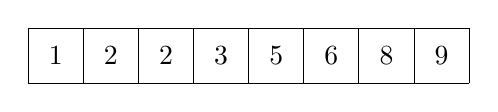
\begin{tikzpicture}[scale=0.7]
\draw (0,0) grid (8,1);
\node at (0.5,0.5) {$1$};
\node at (1.5,0.5) {$2$};
\node at (2.5,0.5) {$2$};
\node at (3.5,0.5) {$3$};
\node at (4.5,0.5) {$5$};
\node at (5.5,0.5) {$6$};
\node at (6.5,0.5) {$8$};
\node at (7.5,0.5) {$9$};
\end{tikzpicture}
\end{center}

\subsubsection{Cận dưới của sắp xếp}

Liệu có thể sắp xếp một mảng nhanh hơn
thời gian $O(n \log n)$ không?
Hóa ra điều này là \emph{không} thể
khi chúng ta chỉ giới hạn ở các thuật toán sắp xếp
dựa trên việc so sánh các phần tử mảng.

Cận dưới cho độ phức tạp thời gian
có thể được chứng minh bằng cách xem việc sắp xếp
như một quá trình trong đó mỗi phép so sánh hai phần tử
cung cấp thêm thông tin về nội dung của mảng.
Quá trình này tạo ra cây sau:

\begin{center}
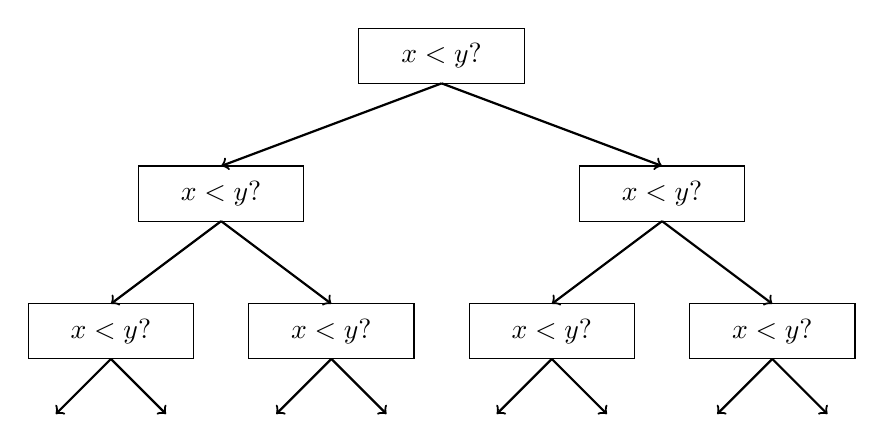
\begin{tikzpicture}[scale=0.7]
\draw (0,0) rectangle (3,1);
\node at (1.5,0.5) {$x < y?$};

\draw[thick,->] (1.5,0) -- (-2.5,-1.5);
\draw[thick,->] (1.5,0) -- (5.5,-1.5);

\draw (-4,-2.5) rectangle (-1,-1.5);
\draw (4,-2.5) rectangle (7,-1.5);
\node at (-2.5,-2) {$x < y?$};
\node at (5.5,-2) {$x < y?$};

\draw[thick,->] (-2.5,-2.5) -- (-4.5,-4);
\draw[thick,->] (-2.5,-2.5) -- (-0.5,-4);
\draw[thick,->] (5.5,-2.5) -- (3.5,-4);
\draw[thick,->] (5.5,-2.5) -- (7.5,-4);

\draw (-6,-5) rectangle (-3,-4);
\draw (-2,-5) rectangle (1,-4);
\draw (2,-5) rectangle (5,-4);
\draw (6,-5) rectangle (9,-4);
\node at (-4.5,-4.5) {$x < y?$};
\node at (-0.5,-4.5) {$x < y?$};
\node at (3.5,-4.5) {$x < y?$};
\node at (7.5,-4.5) {$x < y?$};

\draw[thick,->] (-4.5,-5) -- (-5.5,-6);
\draw[thick,->] (-4.5,-5) -- (-3.5,-6);
\draw[thick,->] (-0.5,-5) -- (0.5,-6);
\draw[thick,->] (-0.5,-5) -- (-1.5,-6);
\draw[thick,->] (3.5,-5) -- (2.5,-6);
\draw[thick,->] (3.5,-5) -- (4.5,-6);
\draw[thick,->] (7.5,-5) -- (6.5,-6);
\draw[thick,->] (7.5,-5) -- (8.5,-6);
\end{tikzpicture}
\end{center}

Ở đây ''$x<y?$'' có nghĩa là một số phần tử
$x$ và $y$ được so sánh.
Nếu $x<y$, quá trình tiếp tục sang trái,
và ngược lại thì sang phải.
Kết quả của quá trình là các cách có thể
để sắp xếp mảng, tổng cộng có $n!$ cách.
Vì lý do này, chiều cao của cây
phải ít nhất là
\[ \log_2(n!) = \log_2(1)+\log_2(2)+\cdots+\log_2(n).\]
Chúng ta có được một cận dưới cho tổng này
bằng cách chọn $n/2$ phần tử cuối cùng và
thay đổi giá trị của mỗi phần tử thành $\log_2(n/2)$.
Điều này mang lại một ước tính
\[ \log_2(n!) \ge (n/2) \cdot \log_2(n/2),\]
vì vậy chiều cao của cây và số bước tối thiểu
có thể có trong một thuật toán sắp xếp
trong trường hợp xấu nhất
ít nhất là $n \log n$.

\subsubsection{Sắp xếp đếm phân phối}

\index{sắp xếp đếm phân phối}

Cận dưới $n \log n$ không áp dụng cho
các thuật toán không so sánh các phần tử mảng
mà sử dụng một số thông tin khác.
Một ví dụ về thuật toán như vậy là
\key{sắp xếp đếm phân phối} (counting sort) sắp xếp một mảng trong
thời gian $O(n)$ với giả định rằng mọi phần tử trong mảng
là một số nguyên trong khoảng $0 \ldots c$ và $c=O(n)$.

Thuật toán tạo ra một mảng \emph{đánh dấu},
mà các chỉ số của nó là các phần tử của mảng ban đầu.
Thuật toán lặp qua mảng ban đầu
và tính toán số lần mỗi phần tử
xuất hiện trong mảng.

Ví dụ, mảng
\begin{center}
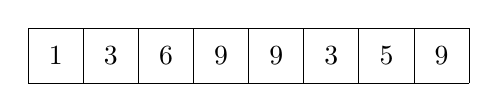
\begin{tikzpicture}[scale=0.7]
\draw (0,0) grid (8,1);
\node at (0.5,0.5) {$1$};
\node at (1.5,0.5) {$3$};
\node at (2.5,0.5) {$6$};
\node at (3.5,0.5) {$9$};
\node at (4.5,0.5) {$9$};
\node at (5.5,0.5) {$3$};
\node at (6.5,0.5) {$5$};
\node at (7.5,0.5) {$9$};
\end{tikzpicture}
\end{center}
tương ứng với mảng đánh dấu sau:
\begin{center}
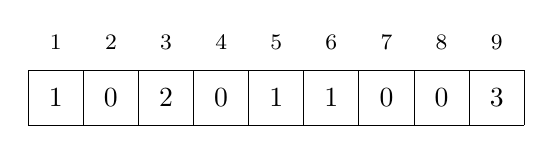
\begin{tikzpicture}[scale=0.7]
\draw (0,0) grid (9,1);
\node at (0.5,0.5) {$1$};
\node at (1.5,0.5) {$0$};
\node at (2.5,0.5) {$2$};
\node at (3.5,0.5) {$0$};
\node at (4.5,0.5) {$1$};
\node at (5.5,0.5) {$1$};
\node at (6.5,0.5) {$0$};
\node at (7.5,0.5) {$0$};
\node at (8.5,0.5) {$3$};

\footnotesize

\node at (0.5,1.5) {$1$};
\node at (1.5,1.5) {$2$};
\node at (2.5,1.5) {$3$};
\node at (3.5,1.5) {$4$};
\node at (4.5,1.5) {$5$};
\node at (5.5,1.5) {$6$};
\node at (6.5,1.5) {$7$};
\node at (7.5,1.5) {$8$};
\node at (8.5,1.5) {$9$};
\end{tikzpicture}
\end{center}

Ví dụ, giá trị tại vị trí 3
trong mảng đánh dấu là 2,
bởi vì phần tử 3 xuất hiện 2 lần
trong mảng ban đầu.

Việc xây dựng mảng đánh dấu
mất thời gian $O(n)$. Sau đó, mảng đã sắp xếp
có thể được tạo ra trong thời gian $O(n)$ vì
số lần xuất hiện của mỗi phần tử có thể được lấy ra
từ mảng đánh dấu.
Do đó, tổng độ phức tạp thời gian của sắp xếp đếm phân phối
là $O(n)$.

Sắp xếp đếm phân phối là một thuật toán rất hiệu quả
nhưng nó chỉ có thể được sử dụng khi hằng số $c$
đủ nhỏ, để các phần tử mảng có thể
được sử dụng làm chỉ số trong mảng đánh dấu.

\section{Sắp xếp trong C++}

\index{sort@\texttt{sort}}

Hầu như không bao giờ là một ý tưởng tốt khi sử dụng
một thuật toán sắp xếp tự viết
trong một cuộc thi, bởi vì có những
cài đặt tốt có sẵn trong các ngôn ngữ lập trình.
Ví dụ, thư viện chuẩn C++ chứa
hàm \texttt{sort} có thể dễ dàng được sử dụng để
sắp xếp mảng và các cấu trúc dữ liệu khác.

Có nhiều lợi ích trong việc sử dụng một hàm thư viện.
Thứ nhất, nó tiết kiệm thời gian vì không cần phải
cài đặt hàm.
Thứ hai, việc cài đặt của thư viện
chắc chắn là đúng và hiệu quả: không có khả năng
một hàm sắp xếp tự viết sẽ tốt hơn.

Trong phần này, chúng ta sẽ xem cách sử dụng
hàm \texttt{sort} của C++.
Đoạn mã sau sắp xếp
một vector theo thứ tự tăng dần:
\begin{lstlisting}
vector<int> v = {4,2,5,3,5,8,3};
sort(v.begin(),v.end());
\end{lstlisting}
Sau khi sắp xếp, nội dung của
vector sẽ là
$[2,3,3,4,5,5,8]$.
Thứ tự sắp xếp mặc định là tăng dần,
nhưng có thể sắp xếp theo thứ tự ngược lại như sau:
\begin{lstlisting}
sort(v.rbegin(),v.rend());
\end{lstlisting}
Một mảng thông thường có thể được sắp xếp như sau:
\begin{lstlisting}
int n = 7; // kich thuoc mang
int a[] = {4,2,5,3,5,8,3};
sort(a,a+n);
\end{lstlisting}
Đoạn mã sau sắp xếp chuỗi \texttt{s}:
\begin{lstlisting}
string s = "monkey";
sort(s.begin(), s.end());
\end{lstlisting}
Sắp xếp một chuỗi có nghĩa là các ký tự
của chuỗi được sắp xếp.
Ví dụ, chuỗi ''monkey'' trở thành ''ekmnoy''.

\subsubsection{Toán tử so sánh}

\index{toán tử so sánh}

Hàm \texttt{sort} yêu cầu
một \key{toán tử so sánh} được định nghĩa cho kiểu dữ liệu
của các phần tử cần sắp xếp.
Khi sắp xếp, toán tử này sẽ được sử dụng
bất cứ khi nào cần phải biết thứ tự của hai phần tử.

Hầu hết các kiểu dữ liệu C++ đều có một toán tử so sánh tích hợp,
và các phần tử của các kiểu đó có thể được sắp xếp tự động.
Ví dụ, các số được sắp xếp theo giá trị của chúng
và các chuỗi được sắp xếp theo thứ tự chữ cái.

\index{pair@\texttt{pair}}

Cặp (\texttt{pair}) được sắp xếp chủ yếu theo
phần tử đầu tiên của chúng (\texttt{first}).
Tuy nhiên, nếu phần tử đầu tiên của hai cặp bằng nhau,
chúng được sắp xếp theo phần tử thứ hai của chúng (\texttt{second}):
\begin{lstlisting}
vector<pair<int,int>> v;
v.push_back({1,5});
v.push_back({2,3});
v.push_back({1,2});
sort(v.begin(), v.end());
\end{lstlisting}
Sau đó, thứ tự của các cặp là
$(1,2)$, $(1,5)$ và $(2,3)$.

\index{tuple@\texttt{tuple}}

Tương tự, bộ (\texttt{tuple})
được sắp xếp chủ yếu theo phần tử đầu tiên,
thứ yếu theo phần tử thứ hai, v.v.
\footnote{Lưu ý rằng trong một số trình biên dịch cũ hơn,
hàm \texttt{make\_tuple} phải được sử dụng để tạo một tuple thay vì
dấu ngoặc nhọn (ví dụ, \texttt{make\_tuple(2,1,4)} thay vì \texttt{\{2,1,4\}}).}:
\begin{lstlisting}
vector<tuple<int,int,int>> v;
v.push_back({2,1,4});
v.push_back({1,5,3});
v.push_back({2,1,3});
sort(v.begin(), v.end());
\end{lstlisting}
Sau đó, thứ tự của các bộ là
$(1,5,3)$, $(2,1,3)$ và $(2,1,4)$.

\subsubsection{Struct do người dùng định nghĩa}

Struct do người dùng định nghĩa không có toán tử
so sánh tự động.
Toán tử này nên được định nghĩa bên trong
struct dưới dạng một hàm
\texttt{operator<},
có tham số là một phần tử khác cùng kiểu.
Toán tử nên trả về \texttt{true}
nếu phần tử hiện tại nhỏ hơn tham số,
và \texttt{false} trong trường hợp ngược lại.

Ví dụ, struct \texttt{P} sau đây
chứa tọa độ x và y của một điểm.
Toán tử so sánh được định nghĩa sao cho
các điểm được sắp xếp chủ yếu theo tọa độ x
và thứ yếu theo tọa độ y.

\begin{lstlisting}
struct P {
    int x, y;
    bool operator<(const P &p) {
        if (x != p.x) return x < p.x;
        else return y < p.y;
    }
};
\end{lstlisting}

\subsubsection{Hàm so sánh}

\index{hàm so sánh}

Cũng có thể cung cấp một
\key{hàm so sánh} bên ngoài cho hàm \texttt{sort}
dưới dạng một hàm callback.
Ví dụ, hàm so sánh \texttt{comp} sau đây
sắp xếp các chuỗi chủ yếu theo độ dài và thứ yếu
theo thứ tự chữ cái:

\begin{lstlisting}
bool comp(string a, string b) {
    if (a.size() != b.size()) return a.size() < b.size();
    return a < b;
}
\end{lstlisting}
Bây giờ một vector chuỗi có thể được sắp xếp như sau:
\begin{lstlisting}
sort(v.begin(), v.end(), comp);
\end{lstlisting}

\section{Tìm kiếm nhị phân}

\index{tìm kiếm nhị phân}

Một phương pháp chung để tìm kiếm một phần tử
trong một mảng là sử dụng một vòng lặp \texttt{for}
lặp qua các phần tử của mảng.
Ví dụ, đoạn mã sau tìm kiếm
một phần tử $x$ trong một mảng:

\begin{lstlisting}
for (int i = 0; i < n; i++) {
    if (array[i] == x) {
        // tim thay x tai chi so i
    }
}
\end{lstlisting}

Độ phức tạp thời gian của phương pháp này là $O(n)$,
bởi vì trong trường hợp xấu nhất, cần phải kiểm tra
tất cả các phần tử của mảng.
Nếu thứ tự của các phần tử là tùy ý,
đây cũng là phương pháp tốt nhất có thể, bởi vì
không có thông tin bổ sung nào cho biết
chúng ta nên tìm kiếm phần tử $x$ ở đâu trong mảng.

Tuy nhiên, nếu mảng đã được \emph{sắp xếp},
tình hình sẽ khác.
Trong trường hợp này, có thể thực hiện
tìm kiếm nhanh hơn nhiều, bởi vì thứ tự của các
phần tử trong mảng sẽ hướng dẫn việc tìm kiếm.
Thuật toán \key{tìm kiếm nhị phân} sau đây
tìm kiếm một phần tử trong một mảng đã sắp xếp một cách hiệu quả
trong thời gian $O(\log n)$.

\subsubsection{Phương pháp 1}

Cách thông thường để cài đặt tìm kiếm nhị phân
giống như tìm một từ trong từ điển.
Việc tìm kiếm duy trì một vùng hoạt động trong mảng,
ban đầu chứa tất cả các phần tử của mảng.
Sau đó, một số bước được thực hiện,
mỗi bước giảm một nửa kích thước của vùng.

Ở mỗi bước, việc tìm kiếm kiểm tra phần tử ở giữa
của vùng hoạt động.
Nếu phần tử ở giữa là phần tử mục tiêu,
việc tìm kiếm kết thúc.
Ngược lại, việc tìm kiếm tiếp tục đệ quy
sang nửa bên trái hoặc bên phải của vùng,
tùy thuộc vào giá trị của phần tử ở giữa.

Ý tưởng trên có thể được cài đặt như sau:
\begin{lstlisting}
int a = 0, b = n-1;
while (a <= b) {
    int k = (a+b)/2;
    if (array[k] == x) {
        // tim thay x tai chi so k
    }
    if (array[k] > x) b = k-1;
    else a = k+1;
}
\end{lstlisting}

Trong cài đặt này, vùng hoạt động là $a \ldots b$,
và ban đầu vùng là $0 \ldots n-1$.
Thuật toán giảm một nửa kích thước của vùng ở mỗi bước,
vì vậy độ phức tạp thời gian là $O(\log n)$.

\subsubsection{Phương pháp 2}

Một phương pháp khác để cài đặt tìm kiếm nhị phân
dựa trên một cách hiệu quả để lặp qua
các phần tử của mảng.
Ý tưởng là thực hiện các bước nhảy và giảm tốc độ
khi chúng ta đến gần phần tử mục tiêu.

Việc tìm kiếm đi qua mảng từ trái sang
phải, và độ dài bước nhảy ban đầu là $n/2$.
Ở mỗi bước, độ dài bước nhảy sẽ được giảm một nửa:
đầu tiên là $n/4$, sau đó là $n/8$, $n/16$, v.v., cho đến khi
cuối cùng độ dài là 1.
Sau các bước nhảy, hoặc phần tử mục tiêu đã
được tìm thấy hoặc chúng ta biết rằng nó không xuất hiện trong mảng.

Đoạn mã sau cài đặt ý tưởng trên:
\begin{lstlisting}
int k = 0;
for (int b = n/2; b >= 1; b /= 2) {
    while (k+b < n && array[k+b] <= x) k += b;
}
if (array[k] == x) {
    // tim thay x tai chi so k
}
\end{lstlisting}

Trong quá trình tìm kiếm, biến $b$
chứa độ dài bước nhảy hiện tại.
Độ phức tạp thời gian của thuật toán là $O(\log n)$,
bởi vì đoạn mã trong vòng lặp \texttt{while}
được thực hiện nhiều nhất hai lần cho mỗi độ dài bước nhảy.

\subsubsection{Các hàm C++}

Thư viện chuẩn C++ chứa các hàm sau đây
dựa trên tìm kiếm nhị phân và hoạt động trong thời gian logarit:

\begin{itemize}
\item \texttt{lower\_bound} trả về một con trỏ đến
phần tử mảng đầu tiên có giá trị ít nhất là $x$.
\item \texttt{upper\_bound} trả về một con trỏ đến
phần tử mảng đầu tiên có giá trị lớn hơn $x$.
\item \texttt{equal\_range} trả về cả hai con trỏ trên.
\end{itemize}

Các hàm này giả định rằng mảng đã được sắp xếp.
Nếu không có phần tử như vậy, con trỏ trỏ đến
phần tử sau phần tử mảng cuối cùng.
Ví dụ, đoạn mã sau tìm hiểu xem
một mảng có chứa một phần tử có giá trị $x$ hay không:

\begin{lstlisting}
auto k = lower_bound(array,array+n,x)-array;
if (k < n && array[k] == x) {
    // tim thay x tai chi so k
}
\end{lstlisting}

Sau đó, đoạn mã sau đếm số lượng phần tử
có giá trị là $x$:

\begin{lstlisting}
auto a = lower_bound(array, array+n, x);
auto b = upper_bound(array, array+n, x);
cout << b-a << "\n";
\end{lstlisting}

Sử dụng \texttt{equal\_range}, đoạn mã trở nên ngắn hơn:

\begin{lstlisting}
auto r = equal_range(array, array+n, x);
cout << r.second-r.first << "\n";
\end{lstlisting}

\subsubsection{Tìm nghiệm nhỏ nhất}

Một ứng dụng quan trọng của tìm kiếm nhị phân là
để tìm vị trí mà giá trị của một \emph{hàm} thay đổi.
Giả sử chúng ta muốn tìm giá trị nhỏ nhất $k$
là một nghiệm hợp lệ cho một bài toán.
Chúng ta được cho một hàm $\texttt{ok}(x)$
trả về \texttt{true} nếu $x$ là một nghiệm hợp lệ
và \texttt{false} trong trường hợp ngược lại.
Ngoài ra, chúng ta biết rằng $\texttt{ok}(x)$ là \texttt{false}
khi $x<k$ và \texttt{true} khi $x \ge k$.
Tình huống trông như sau:

\begin{center}
\begin{tabular}{r|rrrrrrrr}
$x$ & 0 & 1 & $\cdots$ & $k-1$ & $k$ & $k+1$ & $\cdots$ \\
\hline
$\texttt{ok}(x)$ & \texttt{false} & \texttt{false}
& $\cdots$ & \texttt{false} & \texttt{true} & \texttt{true} & $\cdots$ \\
\end{tabular}
\end{center}

\noindent
Bây giờ, giá trị của $k$ có thể được tìm thấy bằng tìm kiếm nhị phân:

\begin{lstlisting}
int x = -1;
for (int b = z; b >= 1; b /= 2) {
    while (!ok(x+b)) x += b;
}
int k = x+1;
\end{lstlisting}

Việc tìm kiếm tìm giá trị lớn nhất của $x$ mà
$\texttt{ok}(x)$ là \texttt{false}.
Do đó, giá trị tiếp theo $k=x+1$
là giá trị nhỏ nhất có thể mà
$\texttt{ok}(k)$ là \texttt{true}.
Độ dài bước nhảy ban đầu $z$ phải
đủ lớn, ví dụ một giá trị nào đó
mà chúng ta biết trước rằng $\texttt{ok}(z)$ là \texttt{true}.

Thuật toán gọi hàm \texttt{ok}
$O(\log z)$ lần, vì vậy tổng độ phức tạp thời gian
phụ thuộc vào hàm \texttt{ok}.
Ví dụ, nếu hàm hoạt động trong thời gian $O(n)$,
tổng độ phức tạp thời gian là $O(n \log z)$.

\subsubsection{Tìm giá trị lớn nhất}

Tìm kiếm nhị phân cũng có thể được sử dụng để tìm
giá trị lớn nhất cho một hàm
ban đầu tăng và sau đó giảm.
Nhiệm vụ của chúng ta là tìm một vị trí $k$ sao cho

\begin{itemize}
\item
$f(x)<f(x+1)$ khi $x<k$, và
\item
$f(x)>f(x+1)$ khi $x \ge k$.
\end{itemize}

Ý tưởng là sử dụng tìm kiếm nhị phân
để tìm giá trị lớn nhất của $x$
mà $f(x)<f(x+1)$.
Điều này ngụ ý rằng $k=x+1$
bởi vì $f(x+1)>f(x+2)$.
Đoạn mã sau cài đặt việc tìm kiếm: 

\begin{lstlisting}
int x = -1;
for (int b = z; b >= 1; b /= 2) {
    while (f(x+b) < f(x+b+1)) x += b;
}
int k = x+1;
\end{lstlisting}

Lưu ý rằng không giống như trong tìm kiếm nhị phân thông thường,
ở đây không được phép các giá trị liên tiếp
của hàm bằng nhau.
Trong trường hợp đó sẽ không thể biết
cách tiếp tục tìm kiếm.